\section{基于结构--温度分解的 SOLAR-H 溶解度预测模型}\label{sec:solar-method}

\subsection{设计动机}

在物理化学中，物质在溶剂中的溶解过程本质上受固液相平衡热力学所支配。根据经典 van 't Hoff 方程，摩尔溶解度随温度的变化由表观溶解焓 $\Delta H_{\mathrm{sol}}$ 调控：
\begin{equation}
\frac{\partial \ln S}{\partial (1/T)} = -\frac{\Delta H_{\mathrm{sol}}}{R},
\end{equation}
在有限的工业操作温区内，一阶局部泰勒近似表明对数溶解度与温度偏离基准值的位移量呈现近似线性依赖。更关键的是，$\Delta H_{\mathrm{sol}}$ 的大小直接由溶质分子与溶剂分子之间的溶剂化作用力与溶质晶格能的差额决定，具有强烈的化学结构特异性。

常规回归方法若直接将温度与高维分子特征并列输入黑盒模型，由于温度仅占单一维度且各组合测量温区不一，算法极易将温度变化与不同分子母体间的溶解度绝对水平发生混淆，导致学到的温度响应在未见母体上严重漂移。为此，本文设计了 SOLAR-H（Structured Orthogonal Linear \& Additive Regression -- Hybrid）模型，其核心思想是解耦预测目标：利用同一化学组合内部的温度变化正交估计局部温度响应斜率，继而在扣除温度项的基准目标上由树集成专门拟合分子结构基线。

\subsection{结构与温度分解}

设第 $i$ 条记录对应的药物--溶剂组合为 $c_i$。为刻画分子结构对温度敏感性的调控，提取药物与溶剂的 11 项基础物理化学描述符（分子量、MolLogP、TPSA、氢键供受体、芳香环数等），经训练折标准化后，构建包含原始值、Hadamard 元素乘积与绝对差值的 44 维结构特征向量 $z_c$。引入偏置项构建增广结构向量 $u_c = [1; z_c] \in \mathbb{R}^{45}$。

以当前训练集的温度中位数 $T_0$ 和四分位距 $s_T$ 对原始温度进行稳健标准化：
\begin{equation}
\tau_i = \frac{T_i - T_0}{s_T},
\end{equation}
SOLAR-H 模型将条件对数溶解度的预测值严密表示为结构基线与温度响应的加性组合：
\begin{equation}\label{eq:v2-solar}
\widehat y_i = b(z_c) + \gamma \cdot \tau_i \cdot \left( u_c^\top \beta \right),
\end{equation}
其中 $b(z_c)$ 表示在基准参考温度（$\tau_i = 0$，即 $T_i = T_0$）下的非线性化学结构基线，由 ExtraTrees 树集成进行拟合；$u_c^\top \beta$ 刻画组合 $c$ 对应的局部温度响应斜率，$\beta \in \mathbb{R}^{45}$ 为待学习的结构调制系数；$\gamma \in [0, 1]$ 为全局温度增益收缩超参数。

\subsection{组内去均值估计}

求解该模型面临的核心难点在于：未知的结构基线 $b(z_c)$ 具有高度复杂的非线性，若直接联合优化，参数 $\beta$ 极易受到分子间巨大溶解度绝对差异的强力干扰。

为解决这一问题，SOLAR-H 借鉴计量经济学面板数据中的固定效应消除技术。对于包含至少两个不同温度测量的训练组合 $c$，定义组内均值 $\bar y_c = \frac{1}{|c|}\sum_{i \in c} y_i$ 与 $\bar\tau_c = \frac{1}{|c|}\sum_{i \in c} \tau_i$。将式\eqref{eq:v2-solar}在组合内取均值并做差：
\begin{equation}
(y_i - \bar y_c) = \left[ b(z_c) - b(z_c) \right] + \gamma (u_c^\top \beta) (\tau_i - \bar\tau_c) + (\varepsilon_i - \bar\varepsilon_c).
\end{equation}
可以看到，复杂的未知非线性项 $b(z_c)$ 在组内差分中被完全数学消除。定义组内离差标签 $\Delta y_i = y_i - \bar y_c$，离差特征向量 $A_i = (\tau_i - \bar\tau_c) u_c^\top \in \mathbb{R}^{45}$。在基准增益 $\gamma = 1$ 下，参数 $\beta$ 的求解被严格转化为带母体加权与 $\ell_2$ 正则化的加权岭回归问题：
\begin{equation}
\widehat\beta = \arg\min_\beta \sum_{i: |\Delta\tau_i| > 0} w_i(q=1) (\Delta y_i - A_i \beta)^2 + \lambda \|\beta\|_2^2.
\end{equation}
令目标函数关于 $\beta$ 的梯度为零，可得严格的闭式解析解：
\begin{equation}
\widehat\beta = (A^\top W A + \lambda I)^{-1} A^\top W \Delta y,
\end{equation}
其中 $W$ 为由母体等权样本权重 $w_i(q=1)$（式\eqref{eq:v2-train-weight}）构成的对角矩阵，$\lambda$ 为岭正则化参数（固定为 1000 以确保高维数值求逆稳定性）。该估计式完全剥离了不同母体分子间的绝对溶解度差异，纯粹利用相同体系受温度驱动的热力学离差，从而获得了对物理温度效应的无偏估计。

\subsection{结构基线与联合求解}

在成功求得温度调制参数 $\widehat\beta$ 后，全量训练样本的温度贡献可被显式计算为 $\widehat\delta_i(\gamma) = \gamma \tau_i u_c^\top \widehat\beta$。随后，构造温度校正后的结构基线学习目标：
\begin{equation}
\widetilde y_i(\gamma) = y_i - \widehat\delta_i(\gamma).
\end{equation}
利用全部训练记录在校正目标 $\widetilde y_i$ 上训练母体等权 ExtraTrees 树集成，作为结构基线函数 $\widehat b(z_c)$。树模型配置 200 棵决策树，叶节点最小样本数为 1。

在内层三折嵌套验证中，联合网格搜索树深上限（8、16、不受限）及温度增益 $\gamma \in \{0, 0.1, 0.3, 1.0\}$，并以母体等权 MAE 为选择准则。选定最优参数后在外层训练集重新拟合，完成端到端联合求解。

\subsection{消融与自适应增益}

为深入探究 SOLAR-H 各核心模块对跨母体泛化性能的贡献，在外层 5 折交叉验证中实施了系统性的消融对比。保持相同的母体划分、测试集与随机种子，分别考察关闭母体加权（$q=0$）、关闭显式交互特征、完全关闭温度项（$\gamma=0$）以及强制满增益（$\gamma=1$）的影响。结果及配对 Bootstrap 95\% 置信区间如图\ref{fig:v2-solar-ablation}所示。

\begin{figure}[htbp]
\centering
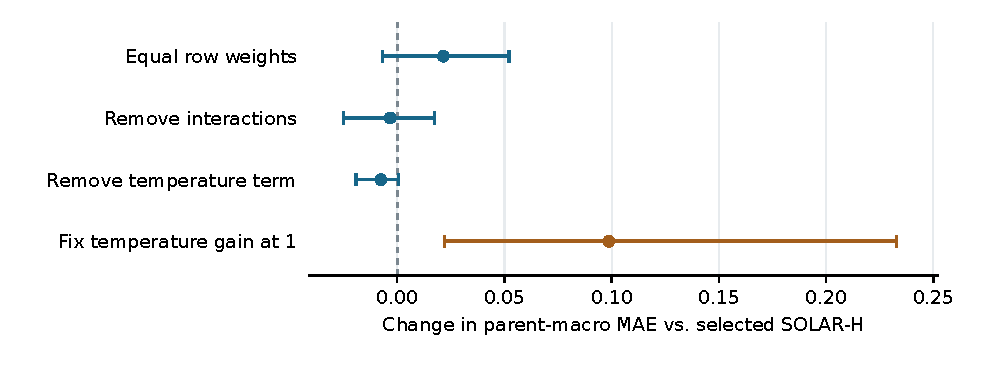
\includegraphics[width=\linewidth]{solar_ablation.pdf}
\caption{SOLAR-H 模型核心机制消融分析。点表示各消融配置相较基准自适应配置的母体等权 MAE 变化量（正值表示误差增加），误差棒表示 10,000 次母体配对 Bootstrap 抽样的 95\% 置信区间。}
\label{fig:v2-solar-ablation}
\end{figure}

消融实验揭示了模型深层的泛化机制。若关闭母体等权加权，SOLAR-H 在未见母体上的 MAE 恶化至 0.7380（上升 0.0216），表明样本重加权是克服高频母体支配、保障稀有母体基线拟合的关键。更为显著的是温度增益的外推效应：当强制设定满增益（$\gamma = 1.0$）时，未见母体 MAE 剧增至 0.8150（性能劣变 0.0987），证实小样本组合的狭窄温区极易受到测定噪声扰动，而内层嵌套自适应选择的收缩阻尼（$\gamma \in \{0, 0.1\}$）能有效抑制过度外推，在学习温度规律的同时确保了外推稳定性。

\subsection{本章小结}

本章构建了兼具热力学可解释性与统计严格性的 SOLAR-H 分解模型，通过组内固定效应消除了结构基线混杂，推导了加权岭回归闭式解，并通过内层嵌套验证确立了自适应增益机制。消融实验不仅验证了各组件的设计合理性，更在方法论层面指出了物理斜率向未知骨架迁移时必须配合自适应阻尼收缩的科学规律。